\documentclass[]{article}

%\usepackage{epcc}
\usepackage{jmlr2e}
%\usepackage[hyphens]{url}
%\PassOptionsToPackage{hyphens}{url}
%\usepackage[colorlinks=false, hidelinks]{hyperref}
\usepackage{amsmath}
\usepackage[toc,page]{appendix}
\usepackage[table]{xcolor}
\usepackage[marginparsep=30pt]{geometry}
\usepackage{stmaryrd}
\usepackage{algorithm}
\usepackage{algorithmic}
\usepackage{tikz}
\usepackage{pgfplots}
\usepackage{tabu}
\usepackage{longtable}
\usepackage{tabularx}
\usepackage{listings}
\usepackage{fancyref}
\usepackage{relsize}
\usepackage{float}
\usepackage{graphicx}
\usepackage{subcaption}
\usepackage{diagbox}
\usepackage{multirow}
\usepackage{slashbox}
\usepackage{graphics}
\usepackage{booktabs}
\usepackage{natbib}
\usepackage{csquotes}

\usetikzlibrary{%
    arrows,
    arrows.meta,
    decorations,
    backgrounds,
    positioning,
    fit,
    petri,
    shadows,
    datavisualization.formats.functions,
    calc,
    shapes,
    shapes.multipart,
    matrix,
    plotmarks
}

\usepgfplotslibrary{fillbetween, statistics, dateplot}

\pgfplotsset{%
  compat=1.3,
  every non boxed x axis/.style={%
  enlarge x limits=false,
  x axis line style={}%-stealth},
  },
  every boxed x axis/.style={},
  every non boxed y axis/.style={%
  enlarge y limits=false,
  y axis line style={}%-stealth},
  },
  every boxed y axis/.style={},
}

\renewcommand{\labelenumii}{\theenumii}
\renewcommand{\theenumii}{\theenumi.\arabic{enumii}.}

\bibliographystyle{plainnat}
\bibpunct{(}{)}{;}{a}{,}{,}

\newenvironment{declaration}
{\centerline{\large\bf Declaration}\vspace{0.7ex}%
  \bgroup\leftskip 20pt\rightskip 20pt\noindent\ignorespaces}%
{\par\egroup\vskip 0.25ex}


\def\title{Deep Learning on SpiNNaker}
\def\author{Jonas Fassbender \\ \textit{jonas@fassbender.dev}}
\date{}

\ShortHeadings{Jonas Fassbender}{\title}

\begin{document}

% titlepage {{{
\begin{titlepage}

\begin{flushleft}
	\vspace*{-1cm}
	
\includegraphics[scale=0.15]{logos/logo_black.pdf}\\
	\vspace*{1cm}
\end{flushleft}
\begin{flushright}
	\vspace*{-3cm}
	
\includegraphics[scale=0.2]{logos/crest_bw.pdf}\\
	\vspace*{1cm}
\end{flushright}


%\EPCCheaderLogos
\null

\begin{center}
\begin{Huge}
\textbf{\title}
\end{Huge}
~\\
~\\
~\\
\textit{\Large {\LARGE M}ASTER {\LARGE T}HESIS}
~\\
~\\
~\\
\begin{Large}
\begin{tabu} to \textwidth {Xr}
Jonas Fassbender
&\href{mailto:jonas@fassbender.dev}{jonas@fassbender.dev}
\end{tabu}
\end{Large}
~\\
~\\
~\\
\begin{large}
In the course of studies

\textit{{\Large H}IGH {\Large P}ERFORMANCE {\Large C}OMPUTING WITH {\Large D}ATA {\Large S}CIENCE}
~\\
~\\
~\\
For the degree of

\textit{{\Large M}ASTER OF {\Large S}CIENCE}
~\\
~\\
~\\
The University of Edinburgh
~\\
~\\
~\\
\begin{tabular}{rl}
  First supervisor: &Caoimhín Laoide-Kemp \\
                    &EPCC, University of Edinburgh \\
  &\\
  Second supervisor: &Dr Kevin Stratford \\
                     &EPCC, University of Edinburgh \\
  &\\
  Third supervisor: &Dr Alan Stokes \\
                    &APT, University of Manchester \\
\end{tabular}
~\\
~\\
~\\
Edinburgh, August 2020
\end{large}
\end{center}
\end{titlepage}
% }}}

\pagenumbering{roman}

% here thanks

% declaration {{{
\hspace{0pt}
\vfill

\begin{declaration}
I declare that this dissertation was composed by myself, that the work
contained herein is my own except where explicitly stated otherwise in
the text, and that this work has not been submitted for any other
degree or professional qualification except as specified.
~\\
~\\
~\\
\begin{tabu}{Xc}
  &Jonas Fassbender \\
  &August 2020
\end{tabu}
\end{declaration}

\vfill
\hspace{0pt}
% }}}

\newpage

% abstract {{{
\hspace{0pt}
\vfill

\begin{abstract}
\end{abstract}

\vfill
\hspace{0pt}
% }}}

\newpage

\tableofcontents

\newpage

\listoffigures

\newpage

\lstlistoflistings

\newpage

% listoftables

\pagenumbering{arabic}

\section{Introduction} % {{{
\label{sec:intro}

Deep learning is revolutionizing the world.
It has become part of our daily lives as consumers, powering major
software products---from recommendation systems and translation tools
to web search \citep{lecun_et_al_2015}.
Major breakthroughs in fields like computer vision
\citep{krizhevsky_et_al_2012} or natural language
processing \citep{hinton_et_al_2012} were achieved through the use of
deep learning.
It has emerged as a driving force behind discoveries in numerous
domains like particle physics \citep{ciodaro_et_al_2012},
drug discovery \citep{ma_et_al_2015}, genomics
\citep{leung_et_al_2014} and gaming \citep{silver_et_al_2016}.

Deep learning has become so ubiquitous that we are changing the
way we build modern hardware to account for its computational demands.
From the way edge devices like mobile phones or embedded systems are
built \citep{deng_2019} and modern CPUs \citep{perez_2017} to
specialized hardware designed only for deep learning models, such
as Google's tensor processing unit (TPU) \citep{jouppi_et_al_2017} or
NVIDIA's EGX Edge AI platform \citep{boitano_2020}.
Whole state-of-the-art supercomputers are built solely for deep
learning.
An example would be a supercomputer built by Microsoft for OpenAI,
which is part of the Azure cloud \citep{langston_2020}.

Hardware manufacturer are faced with a major challenge in meeting the
computational demands arising from inference, and more importantly,
training deep learning models.
OpenAI researchers have estimated that the computational costs of
training increases exponentially; approximately every 3.4 months the
cost doubles \citep{amodei_et_al_2019}.
\citet{amodei_et_al_2019} claims the deep reinforcement learning agent
AlphaGo Zero---the successor of the famous AlphaGo program, which
was able to beat Go world champion Lee Sedol
\citep{silver_et_al_2017}---to be the system  with the highest
computational demands of approximately 1850 petaflop/s-days.
AlphaGo Zero was trained for 40 days on a machine with 4 TPUs
\citep{silver_et_al_2017}.
With the end of Moore's Law \citep{loeffler_2018}, chip makers have to
get creative in scaling up computing, the same way machine learning
researchers are scaling up their models \citep{simonite_2016}.
Therefore production and research into new hardware designs for deep
learning are well on the way.

Another field which has high computational demands for very specific
tasks and algorithms is computational neuroscience.
Computational neuroscience has long been linked to deep learning,
which has its origin in research done by neuroscientists
\citep{goodfellow_et_al_2016, mcculloch_et_al_1943}.
While in the recent past deep learning research has been more focused
on mathematical topics like statistics and probability theory,
optimization or linear algebra, researchers are again looking to
neuroscience to further improve the capabilities of deep
learning models \citep{marblestone_et_al_2016}.

But the algorithms developed by computational neuroscientists are not
the only aspect drawing attention from the deep learning community.
Computational neuroscience has a long standing history of
developing custom hardware for the efficient modeling of the human
brain, so called neuromorphic computing. Neuromorphic computing---a
computer architecture inspired by the biological nervous system---has
been around since the 1980s \citep{mead_1989}.
Today, neuromorphic computers are being developed to meet the
demands for efficient computing needed to run large-scale
spiking neural networks used for modeling brain
functions \citep{furber_2016}.
While being developed mainly for the task of modeling the human brain,
deep learning has been linked to neuromorphic computing,
especially in the context of commercial usability \citep{gomes_2017}.
Both the low energy demands of neuromorphic computers---such as IBM's
True North \citep{cassidy_et_al_2013} or The University of
Manchester's Spiking Neural Network Architecture (SpiNNaker)
\citep{furber_et_al_2006}---and their
scalability and massive-parallelism are intriguing for two very
important use cases of deep learning:
(\romannumeral 1) edge computing, for example robotics
and mobile devices, (\romannumeral 2) supercomputers and the
cloud-era \citep{gomes_2017}.

This thesis investigates the performance of SpiNNaker machines for
deep learning by training the state-of-the-art computer vision model
ResNet-50 \citep{he_et_al_2015} under the closed division rules of the
MLPerf training benchmark \citep{mattson_et_al_2019}.
In order to benchmark ResNet-50 on SpiNNaker a prototypical
implementation was developed as part of this thesis.

\begin{itemize}
  \item here a paragraph about the results
\end{itemize}

Section~\ref{sec:background} presents the background of this thesis.
An introduction to deep learning is given in
Section~\ref{subsec:intro_dl}, as well as an overview
of the benchmark in Section~\ref{subsec:intro_bench}.
Section~\ref{subsec:intro_spinn} describes the SpiNNaker architecture
and compares it to current deep learning hardware.
Related work can be found in Section~\ref{sec:related_work}.
Section~\ref{sec:SpiDNN} presents the architecture of the
prototype developed for benchmarking and Section~\ref{sec:benchmark}
presents the benchmarks and its results.
In Section~\ref{sec:discussion} the results of the benchmark are
discussed, as well as the development process.
Section~\ref{sec:conclusion} contains the conclusion, while
Section~\ref{sec:next_steps} outlines the next steps for further
increasing the performance of SpiNNaker by enhancing the
prototype.

% }}}


\section{Background} % {{{
\label{sec:background}

This section summarizes the background knowledge needed for the
following sections.
First a short introduction to deep learning is given in
Section~\ref{subsec:intro_dl}.
The main focus lies on the basic concepts and those concepts important
for computer vision.
Next, Section~\ref{subsec:intro_bench} outlines the context of the
conducted benchmark presented in Section~\ref{sec:benchmark}.
Lastly, the SpiNNaker neuromorphic computer architecture is described
in Section~\ref{subsec:intro_spinn}.
SpiNNaker is also compared against the two state-of-the-art hardware
solutions for deep learning that currently produce the best
performance in training and inference.
Namely general purpose graphical processing units (GPGPUs) and
Google's tensor processing unit (TPU).

\subsection{An Introduction to Deep Learning} % {{{
\label{subsec:intro_dl}

While it may seem that deep learning is a recent development in the
field of artificial intelligence---due to all the recently announced
breakthroughs \citep{senior_et_al_2020, vinyals_et_al_2019,
  openai_2019, margi_2019}---it has actually existed since the 1940s
\citep{goodfellow_et_al_2016}.
\citet{mcculloch_et_al_1943} first described the McCulloch-Pitts
neuron as a simple mathematical model of a biological neuron, which
marks the origin of what is known today as deep learning.

Even though deep learning models today are still called
\textit{artificial neural networks} (due to their historical context),
they are quite different from \textit{spiking neural networks}
(which SpiNNaker was designed to run efficiently).
While the former has been described as ``just nonlinear statistical
models'' \citep{hastie_et_al_2009}, the latter incorporated findings
about biological neurons and is therefore more closely related to how
the nervous system works \citep{maass1997}.
Spiking neural networks are mostly used for simulation, unlike deep
learning models, which are mostly used for inference.

The history of deep learning can be broken down into three distinct
phases.
Only during the last of these phases was the methodology
called deep learning \citep{goodfellow_et_al_2016}.
Arguably the reason why deep learning seems to be a new development.
The first phase, where deep learning was known as cybernetics, ranged
from the 1940s to the 1960s \citep{goodfellow_et_al_2016}.
As stated above, it was the time when the first biologically
inspired representations of neurons were developed.
\citet{rosenblatt_1958} presents the first model, a single trainable
artificial neuron known as the perceptron (see
Figure~\ref{fig:perceptron}).

Today's perceptron receives a real-valued $n$-vector $\mathbf{x}$ of
\textit{input} signals and builds the dot product with another
real-valued $n$-vector known as \textit{weights} $\mathbf{w}$:
$\mathbf{x}\cdot\mathbf{w} = \sum_{i=1}^{n}x_iw_i$.
The \textit{bias} $b$ is added to the dot product.
$\mathbf{x} \cdot \mathbf{w} + b$ is then passed to the
\textit{activation function} $g$---some fixed transformation function
appropriate for the application domain.
$y = g(\mathbf{x} \cdot \mathbf{w} + b)$ is the output of the
perceptron.

During \textit{supervised learning}, we have a set of
\textit{examples}.
Each example consists of an \textit{input} vector $\mathbf{x}$ and a
associated \textit{label} $y$ generated by an unknown function
$f^*(\mathbf{x})$.
A perceptron can be trained to approximate $f^*(\mathbf{x})$.
We can describe a perceptron as the mathematical function
\begin{align}
  \label{eq:perceptron}
  y = f(\mathbf{x};\mathbf{w}, b) = g(\mathbf{x} \cdot \mathbf{w} + b).
\end{align}
$f(\mathbf{x};\mathbf{w}, b)$ is known as a
\textit{(statistical) model} with
$\mathbf{w}$ and $b$ as its \textit{trainable parameters},
which are trained/learned in order to approximate $f^*$ with $f$.
How a network of perceptrons---a more complex statistical model better
suited for real world applications---is trained via backpropagation
and gradient descent, will be explained below.

\begin{figure} % {{{
	\begin{center}
	\begin{tikzpicture}[dot/.style={circle,draw}]
		\node at (3,0) (out) {$y$};
		\node at (0,0) [dot] (neuron) {$\mathbf{x} \cdot \mathbf{w} + b$}
			edge[->] node[above]{$g$} (out);
		\node at (-3,4) [dot] {$x_1$}
			edge[->] (neuron);
		\node at (-3,2) [dot] {$x_2$}
			edge[->] (neuron);
		\node at (-3,0) [dot] {$x_3$}
			edge[->] (neuron);
		\node at (-3,-4) [dot] {$x_n$}
			edge[->] (neuron);
		\node at (-3,-2) [] {\vdots};
	\end{tikzpicture}
	\end{center}
	\caption {Schema of a perceptron.}
	\label{fig:perceptron}
\end{figure} % }}}

The second historical phase of deep learning is known as
connectionism (1980s-1990s) \citep{goodfellow_et_al_2016}.
Its main contributions to today's knowledge were the backpropagation
algorithm \citep{rumelhart_et_al_1986} and the approach of parallel
distributed processing
\citep{rumelhart_et_al_1986a, rumelhart_et_al_1986b}, which provided a
mathematical framework around the idea that a large number of simple
computational units (e.g.\ the perceptron) could achieve intelligent
behavior when connected together \citep{goodfellow_et_al_2016}.
Backpropagation enabled the training of networks of
perceptrons---artificial neural networks.

The quintessential artificial neural network is the \textit{multilayer
perceptron} (MLP), also called a \textit{feedforward neural network}
(see Figure~\ref{fig:mlp}) \citep{goodfellow_et_al_2016}.
The MLP consists of multiple perceptrons organized in \textit{layers}.
Layers are connected successively such that the output of each of its
perceptrons reaches all perceptrons in the next layer.
Such a layer is known to be \textit{fully-connected} or
\textit{dense}. No cycle exists between perceptrons; the MLP is a
directed acyclic graph.
Unlike the single layer perceptron, the MLP has at least one
\textit{hidden layer}.
A hidden layer is a layer between the input and output layers (see
Figure~\ref{fig:mlp}).

\begin{figure} % {{{
\begin{center}
	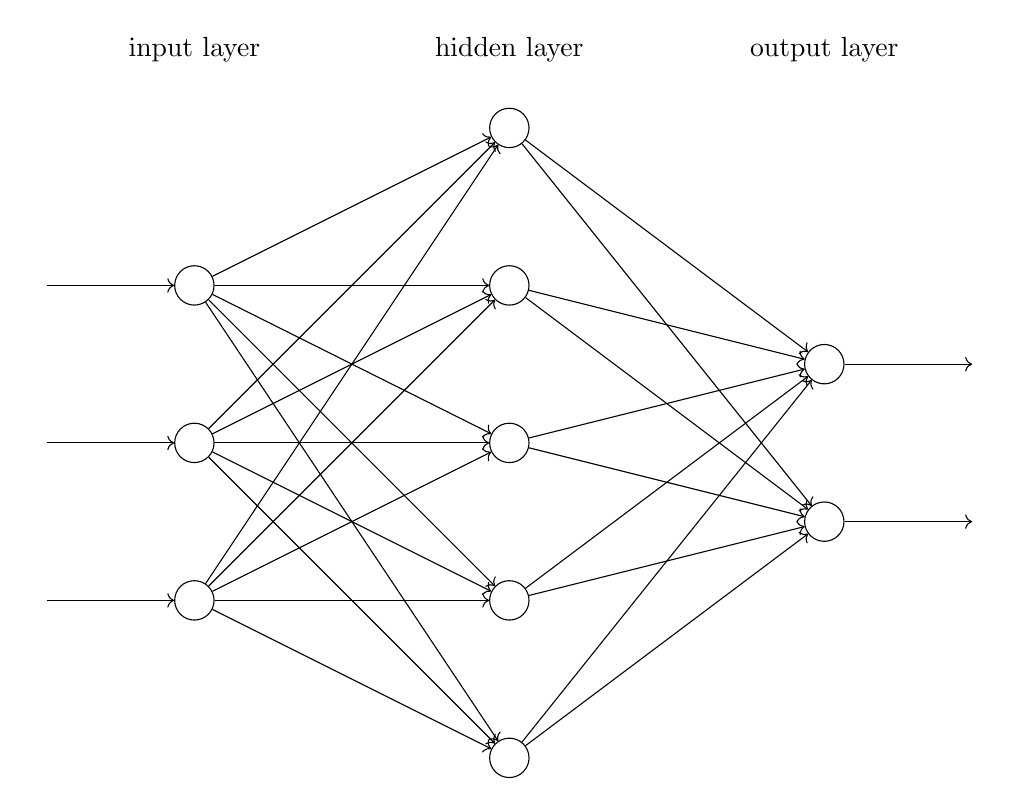
\begin{tikzpicture}[dot/.style={circle,draw,minimum size = .5cm}]
		\node at(-4,5) {input layer};
		\node at(0,5) {hidden layer};
		\node at(4,5) {output layer};

		\node at(6,1) (oo1) {};
		\node at(6,-1) (oo2) {};

		\node at (4,1) [dot] (o1) {}
			edge[->] (oo1);
		\node at (4,-1) [dot] (o2) {}
			edge[->] (oo2);

		\node at (0,4) [dot] (h1) {}
			edge[->] (o1)
			edge[->] (o2);
		\node at (0,2) [dot] (h2) {}
			edge[->] (o1)
			edge[->] (o2);
		\node at (0,0) [dot] (h3) {}
			edge[->] (o1)
			edge[->] (o2);
		\node at (0,-2) [dot] (h4) {}
			edge[->] (o1)
			edge[->] (o2);
		\node at (0,-4) [dot] (h5) {}
			edge[->] (o1)
			edge[->] (o2);

		\node at (-4,2) [dot] (i1) {}
			edge[->] (h1)
			edge[->] (h2)
			edge[->] (h3)
			edge[->] (h4)
			edge[->] (h5);
		\node at (-4,0) [dot] (i2) {}
			edge[->] (h1)
			edge[->] (h2)
			edge[->] (h3)
			edge[->] (h4)
			edge[->] (h5);
		\node at (-4,-2) [dot] (i3) {}
			edge[->] (h1)
			edge[->] (h2)
			edge[->] (h3)
			edge[->] (h4)
			edge[->] (h5);

		\node at(-6,2) (ii1) {}
			edge[->] (i1);
		\node at(-6,0) (ii2) {}
			edge[->] (i2);
		\node at(-6,-2) (ii3) {}
			edge[->] (i3);
	\end{tikzpicture}
\end{center}
\caption {Schema of a MLP or feedforward neural network.}
\label{fig:mlp}
\end{figure} % }}}

A MLP can also be represented as a statistical model
$f(\mathbf{x};\mathbf{\theta})$.
Computing $f(\mathbf{x})$---also called \textit{inference} or the
\textit{forward pass}---can be described as a layer-wise composition
of functions $f^{(1)}, f^{(2)}, \dots, f^{(l)}$, each function
$f^{(i)}, i < l$ being a hidden layer and $f^{(l)}$ being the output
layer.
The perceptron has the weight vector $\mathbf{w}$ and the bias
$b$ as its parameters (see Equation~\ref{eq:perceptron}).
The parameters of a layer are the combination of
$\mathbf{w}$ and $b$ for each of its perceptrons.
For example, if the first hidden layer contains $m$ perceptrons and
$\mathbf{x}$ is a $n$-vector, then the parameters of $f^{(1)}$ would
be a matrix $\mathbf{W}: n \times m$ and a $m$-vector $\mathbf{b}$.
The output of layer $f^{(1)}$ would be a $m$-vector computed as
follows:
\begin{align}
  f^{(1)}(\mathbf{x}; \mathbf{W}, \mathbf{b}) =
  g(\mathbf{W}^\top\mathbf{x} + \mathbf{b}).
\end{align}
The second layer takes the output of the first and so forth.
The forward pass of the MLP is computed as:
\begin{align}
  y = f^{(l)}(f^{(l-1)}(\dots f^{(1)}(\mathbf{x}))).
\end{align}

The backpropagation algorithm is a way to train the parameters of a
MLP (or other deep learning models) so that it approximates the
unknown function $f^*$ which generates the labels of the examples
we have in our data set.
The data set used for training a model is called the \textit{training
set}.
In addition to the training set there normally exists a
\textit{test set} with examples the model has not seen before
(examples not in the training set).
The test set is used to determine the generalization performance of
the model.
Backpropagation is an algorithm that allows to train a deep learning
model with \textit{(stochastic or batch) gradient descent}.
For example, $\hat{y} = f(\mathbf{x})$ and $y$ is the true label
($y$ and $\hat{y}$ are $k$-vectors), the error of $f$ is computed
using a \textit{loss function} $L$, for example mean squared error:
$1/k \sum_{i=1}^{k}(y_k - \hat{y}_k)^2$.
In order to get the gradients of the weights of the output layer
we calculate the derivative of the loss according to each weight
$w_{ij}$ in $\mathbf{W}$ with the chain rule:
\begin{align}
  \frac{\delta L}{\delta w_{ij}} =
    \frac{\delta L}{\delta g}
    \frac{\delta g}{\delta h}
    \frac{\delta h}{\delta w_{ij}},
\end{align}
$h$ being $\mathbf{W}^\top f^{(l-1)} + \mathbf{b}$.
$w_{ij}$ is updated by performing the stochastic gradient descent%
\footnote{Or (batch) gradient descent. With gradient descend the whole
  training set is passed through the MLP before the weights
  are updated with the sum over the loss of each example in the
  training set. Batch or Mini-batch gradient descent takes a subset of
  the whole training set and updates the weights after each
  mini-batch. Deep learning models are normally trained by passing the
  training set multiple times through the model. Each pass over the
  whole training set is called an \textit{epoch}.
}:
\begin{align}
  w_{ij}^+ = w_{ij} - \mu \frac{\delta L}{\delta w_{ij}},
\end{align}
with $\mu$ as the \textit{learning rate}.
The same procedure is applied to the following hidden layers.
The total loss of the next hidden layer is given as:
\begin{align}
  L^{(l-1)} = \sum_{i=1}^n\frac{\delta L}{\delta f^{(l - 1)}_i} =
  \sum_{i=1}^n\frac{\delta L}{\delta g}
    \frac{\delta g}{\delta h}
    \frac{\delta h}{\delta f^{(l - 1)}_i},
\end{align}
$f^{(l-1)}_i$ being the $i$-th perceptron of the hidden layer $l-1$.

\citet{hornik_et_al_1989} demonstrated that a non-linear MLP
(the activation functions are non-linear transformations of
$h(x) = \mathbf{W}^\top\mathbf{x} + \mathbf{b}$) can overcome the
famous XOR problem of a single layer perceptron demonstrated in
\citet{minsky_et_al_1969}.
Another major contribution of the phase of connectionism was the
neocognitron \citep{fukushima_1980}, the origin of today's
\textit{convolutional neural networks} (CNNs)---which are the
state-of-the-art approach for building computer vision models---and
the application of the backpropagation algorithm to fully automate the
training of CNNs \citep{lecun_et_al_1989}.

\citet{goodfellow_et_al_2016} claims that the third and current phase
of deep learning---where the name deep learning was
established---starts with \citet{hinton_et_al_2006} describing a new
learning algorithm called greedy layer-wise pretraining, which they
applied to deep belief networks.
Greedy layer-wise pretraining was soon generalized to work with other
deep artificial neural network architectures
\citep{renzato_et_al_2006, bengio_et_al_2007}.
While these papers may have resulted in the term deep learning,
they were not the reason for the resurrected interest in this
methodology.
The two most important factors are the increase of available data
and computation.
The former enables better generalization
\citep{goodfellow_et_al_2016}, while the latter allows
training bigger models (more hidden layers---the \textit{depth} of the
neural networks increased) which can solve more complex problems
\citep{bengio_et_al_2007a, goodfellow_et_al_2016}.

Like the perceptron, ``neurons'' in a \textit{convolutional layer}
are inspired by findings of neuroscientists.
In this case by research done by Hubel and Wiesel about the
mammalian visual cortex
\citep{hubel_et_al_1959, hubel_et_al_1962, hubel_et_al_1968}.
CNNs are just deep learning models which have at least one
convolutional layer. They are applied to problems which have a
grid-like topology, like time-series (1D), images (2D) or videos (3D)
\citep{goodfellow_et_al_2016}.

Unlike dense layers of perceptrons, convolutional layers do not apply
a full matrix multiplication $\mathbf{W}^\top\mathbf{x}$ but instead
a linear operation $*$ called convolution.
A one dimensional discrete convolution can be described as:
\begin{align}
  \label{eq:conv}
  s(i) = (x * w)(i) = \sum_n x(i + n)w(n).
\end{align}
Equation~\ref{eq:conv} is not really a convolution but is referred to
as \textit{cross-correlation}.
Unlike true convolution, cross-correlation is not commutative
\citep{goodfellow_et_al_2016}.
However, commutativity is not a factor in practice, so many deep
learning libraries, like Keras \citep{keras} or the prototype
developed for this thesis implement cross-correlation rather than true
convolution.
Convolution will refer to cross-correlation below.

In the case of deep learning, $x$ is a $n$D array called the
\textit{input} and $w$ is another $n$D array referred to as the
\textit{kernel}. The kernel elements are the trainable parameters
\citep{goodfellow_et_al_2016}.
In Equation~\ref{eq:conv}, $x$ and $w$ are one dimensional.
If we let $x$ be a $m$-vector, the function $x(i)$ is defined as:
\begin{align}
  \label{eq:valid_conv}
  x(i) = \begin{cases}
    x_i &\text{if } 1 \leq i \leq m \\
    0 &\text{otherwise.}
  \end{cases}
\end{align}
$n$ is the size of the kernel in the first dimension.
Figure~\ref{fig:conv_op} shows an example of how the output of a
1D convolutional layer is computed.
Figure~\ref{fig:cnn} shows the schema of the convolutional
layer performing the operation from Figure~\ref{fig:conv_op}.
The result of a convolution can be transformed by an activation
function like the perceptron and the concept of the bias applies also.

\begin{figure} % {{{
\begin{center}
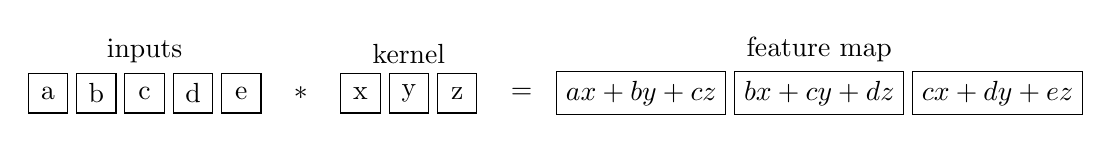
\begin{tikzpicture}[box/.style={rectangle,draw, minimum size=.5cm}]
  \node[box] at (0,0) (a) {a};
  \node[right=.1 of a, box] (b) {b};
  \node[right=.1 of b, box, label=inputs] (c) {c};
  \node[right=.1 of c, box] (d) {d};
  \node[right=.1 of d, box] (e) {e};

  \node[right=.9 of d] {$*$};

  \node[right=1 of e, box] (x) {x};
  \node[right=.1 of x, box, label=kernel] (y) {y};
  \node[right=.1 of y, box] (z) {z};

  \node[right=.3 of z] {$=$};

  \node[right=1 of z, box] (fst) {$ax + by + cz$};
  \node[right=.1 of fst, box, label=feature map] (snd)
    {$bx + cy + dz$};
  \node[right=.1 of snd, box] (trd) {$cx + dy + ez$};
\end{tikzpicture}
\end{center}
\caption{Example of a 1D cross-correlation operation with a kernel
  size of three, a single channel, a single filter, a stride of one
  and valid padding.}
\label{fig:conv_op}
\end{figure} % }}}

\begin{figure} % {{{
\begin{center}
	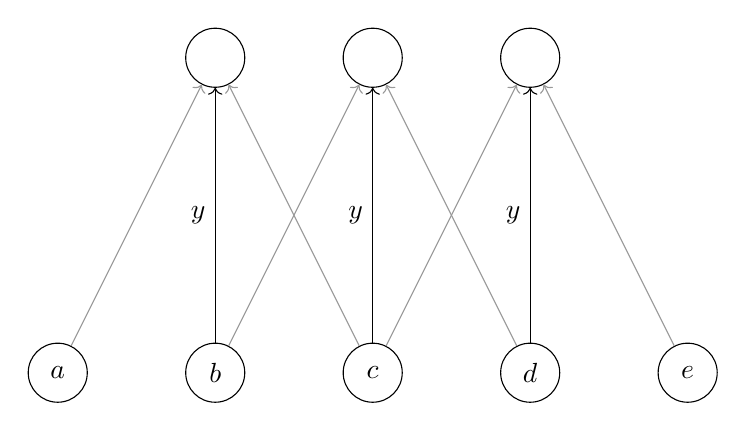
\begin{tikzpicture}[rotate=90, dot/.style={circle,draw,minimum size = .75cm}]
		\node at (0,2) [dot] (h2) {};
		\node at (0,0) [dot] (h3) {};
		\node at (0,-2) [dot] (h4) {};

		\node at (-4,4) [dot] (i1) {$a$}
			edge[black!40, ->] (h2);
		\node at (-4,2) [dot] (i2) {$b$}
			edge[->] (h2)
			edge[black!40, ->] (h3);
		\node at (-4,0) [dot] (i3) {$c$}
			edge[black!40, ->] (h2)
			edge[->] (h3)
			edge[black!40, ->] (h4);
		\node at (-4,-2) [dot] (i4) {$d$}
			edge[black!40, ->] (h3)
			edge[->] (h4);
		\node at (-4,-4) [dot] (i5) {$e$}
			edge[black!40, ->] (h4);

    \node[left] at (-2,2) {$y$};
    \node[left] at (-2,0) {$y$};
    \node[left] at (-2,-2) {$y$};
	\end{tikzpicture}
\end{center}
\caption {Schema for the convolutional layer performing the
  convolution shown in Figure~\ref{fig:conv_op}. Each neuron
  represents one convolution. The schema shows the
  property of shared weights and sparse
  connectivity \citep{goodfellow_et_al_2016}. The black edges
  all have the same associated weight $y$, while one can see that
  there are much less edges compared to a dense layer shown in
  Figure~\ref{fig:mlp}.}
\label{fig:cnn}
\end{figure} % }}}

Normally a convolutional layer does not consist of a single
convolution, but applies multiple kernels to the output of the
previous layer.
A single convolution is called a \textit{filter} and a layer
consists of a predefined number of filters, each with its own kernel
(and optionally a bias) \citep{brownlee_2019}.
The output of a convolutional layer is often called a
\textit{feature map} \citep{goodfellow_et_al_2016}.
Even though an image may seem to be a two dimensional structure of
pixels, in most cases it is actually three dimensional, the third
dimension being the RGB color values for each pixel.
The third dimension of the three RGB colors are called the
\textit{channels} \citep{goodfellow_et_al_2016}.
For example, we have a data set of images with $256\times256$
pixels and three channels (red, green and blue).
We pass the image to a convolutional layer with a $3\times3$ kernel
shape and $64$ filters.
A kernel consists of 18 elements, the kernel size (for the two
spatial dimensions) times the three channels of each pixel.
The shape of the feature map of that layer---if we assume ``same''
padding (see below)---would be $256\times256\times64$, so the
next layer would have 64 channels.

There are two more notable concepts of convolutional layers:
\textit{stride} and \textit{padding}.
The former refers to skipping convolutions in order to reduce the
computational cost at the expense of less exact feature extraction
(patterns may not be detected by the model due to the increased
inaccuracy).
The latter is a way of dealing with vanishing spatial dimensions of
the feature map if we only perform convolutions on ``valid'' inputs
($1 \leq i \leq m$ in Equation~\ref{eq:valid_conv}).
``Valid'' padding refers to the fact that the input has no padding.
The feature map of the convolutional layer will have
its kernel size minus one less neurons than its input
(see Figure~\ref{fig:cnn}).
``Same'' padding would be to add enough zeros evenly above and below
the valid input (along each spatial dimension) so that the feature map
of the convolutional layer will have the same spatial dimensions as
its input (see Figure~\ref{fig:padding} \citep{goodfellow_et_al_2016}.

\begin{figure} % {{{
\begin{center}
	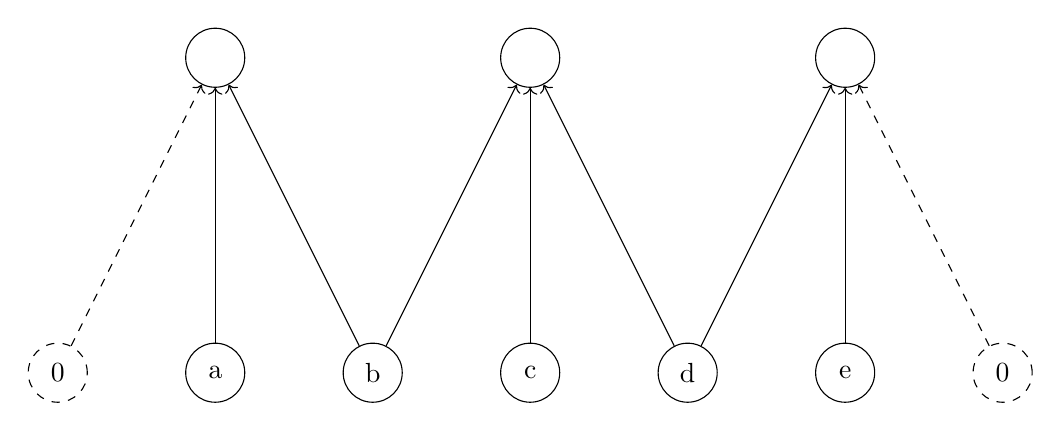
\begin{tikzpicture}[rotate=90, dot/.style={circle,draw,minimum size = .75cm}]
		\node at (0,4) [dot] (h1) {};
		\node at (0,0) [dot] (h3) {};
		\node at (0,-4) [dot] (h5) {};

		\node at (-4,6) [dot, dashed] (i0) {0}
			edge[->, dashed] (h1);
		\node at (-4,4) [dot] (i1) {a}
      edge[->] (h1);
		\node at (-4,2) [dot] (i2) {b}
			edge[->] (h1)
			edge[->] (h3);
		\node at (-4,0) [dot] (i3) {c}
			edge[->] (h3);
		\node at (-4,-2) [dot] (i4) {d}
			edge[->] (h3)
			edge[->] (h5);
		\node at (-4,-4) [dot] (i5) {e}
			edge[->] (h5);
		\node at (-4,-6) [dot, dashed] (i6) {0}
			edge[->, dashed] (h5);
	\end{tikzpicture}
\end{center}
\caption {Example showing a layer with same padding and a
  stride of two.}
\label{fig:padding}
\end{figure} % }}}

Along convolutional layers, CNNs often have \textit{pooling layers}.
A pooling layer summarizes locally with the goal of making the
CNN invariant to small translations of the input
\citep{goodfellow_et_al_2016}, making the model less prone to
\textit{overfitting}---the state a model is in if it performs well
on the training set but does not generalize well to unseen examples.
\textit{Max pooling}, for example, takes some local neighborhood of
the input, exactly like a convolutional layer, and returns the
maximum value of that neighborhood.

% }}}


\subsection{Benchmarking Deep Learning Systems for Computer Vision} % {{{
\label{subsec:intro_bench}

In 2010 the annual (until 2017) ImageNet Large Scale Visual
Recognition Challenge (ILSVRC) was launched and has become the most
famous benchmark for computer vision models, producing many well-known
deep learning models like AlexNet in 2012
\citep{krizhevsky_et_al_2012}, VGG16 in 2014
\citep{simonyan_et_al_2014} and the ResNet models in 2015
\citep{he_et_al_2015}.
The ILSVRC---like the name suggests---is based on the ImageNet data
set consisting of more than 14 million images
\citep{russakovsky_et_al_2015}.
One task of the ILSVRC benchmark is image classification.
During image classification the model is trained on 1000 categories
(1.2 million images), without overlapping labels (each image has a
single label, e.g.~``dog'') \citep{russakovsky_et_al_2015}.
The top-1 ($y = \text{argmax } f(\mathbf{x})$) accuracy is measured on
a test set of 150,000 images and winner is the model with the highest
top-1 accuracy.

While a benchmark like the ILSVRC produces new insights into computer
vision and keeps the community up to date on what is possible,
deep learning has another issue on which a benchmark can shed light:
training/inference speed of hardware and software systems.
The MLPerf benchmark was developed to tackle this problem, so
stakeholders can make informed decisions and to provide the
industry---like hardware vendors, cloud providers and machine learning
engineers---with a fair standard to rely on
\citep{mattson_et_al_2019}.
One task of the MLPerf training benchmark is training the ResNet-50
model (see below) on the image classification task from the ILSVRC
2012, until it reaches a top-1 accuracy of 74.9 percent.
The wallclock time is measured and serves as the result for the
benchmarked system \citep{mattson_et_al_2019}.
Currently the fastest solution, from the latest MLPerf training
benchmark v0.6, is Google's cloud system based on Tensorflow and
one TPUv3 pod (1024 TPUv3s) \citep{mlperf_2019, stone_2019}.
Our benchmark, presented in Section~\ref{sec:benchmark}, is based
on the image classification task of the MLPerf training benchmark,
making it easy to compare SpiNNaker and our prototype to other
state-of-the-art deep learning systems.

The winner of the image classification task of the ILSVRC 2015 was an
ensemble of residual nets (ResNets) introduced in
\citet{he_et_al_2015}.
The ensemble generated a top-5 accuracy (true label in the five
highest outputs of the ensemble) of 96.4 percent.
ResNets are a revolution in the sense that they are not only better
classifiers than previous models, they also can be significantly
deeper \citep{he_et_al_2015}.
\citet{he_et_al_2015} presents a 152-layer deep network, eight times
deeper than a ``very deep convolutional network'' (VGG11--VGG19)
\citep{simonyan_et_al_2014, he_et_al_2015}.
ResNets can be so deep, without losing their ability of convergence
and without degradation (saturated accuracy and higher training error
with increased depth) \citep{he_et_al_2015}, by introducing residual
blocks with shortcut connections (see Figure~\ref{fig:shortcut_conn}).
\citet{he_et_al_2015} hypothesizes that residual blocks ease the
learning of the model.
These shortcut connections do not increase the complexity of the
model. No additional parameters are added to the model and nothing
changes during backpropagation.
Only the negligible operation where $\mathbf{x}$ is added to the
output of the residual block must be performed during the forward
pass.
\citet{he_et_al_2015} shows comprehensive tests on how residual blocks
decrease degradation by comparing ResNets against their
counterparts with the same architecture, but without shortcut
connections.
The models without shortcut connections show a higher training error
than their ResNet counterpart.

\begin{figure}
  \begin{center}
    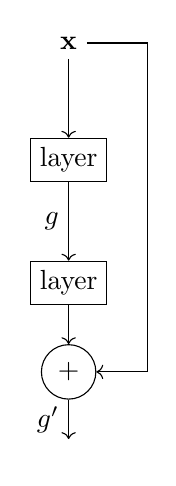
\begin{tikzpicture}
      \node[rectangle, draw] at (0, 0) (layer0) {layer};
      \node[rectangle, draw, below=1 of layer0] (layer1) {layer};
      \node[circle, draw, below=.5 of layer1] (layer_add) {$+$};
      \node[below=.5 of layer_add] (layer_out) {};
      \node[above=1 of layer0] (layer_in) {$\mathbf{x}$};

      \draw[->] (layer_in) -- (layer0);
      \draw[->] (layer0) -- node[left]{$g$} (layer1);
      \draw[->] (layer1) -- (layer_add);
      \draw[->] (layer_add) -- node[left]{$g^\prime$} (layer_out);

      \draw[->] (layer_in) -| ($(layer_add) + (1,0)$) |- (layer_add);
    \end{tikzpicture}
  \end{center}
  \caption{Schema of a residual block with two layers. $\mathbf{x}$ is
    added to the output of the last layer of the residual block,
    before the result is passed through its activation function
    $g^\prime$.}
  \label{fig:shortcut_conn}
\end{figure}

As stated above, the image classification task of the MLPerf
training benchmark is to train ResNet-50 (50, because it has 50
layers) until it reaches a top-1 accuracy of 74.9 percent on the test
set and to measure the wallclock time it took to reach that goal.
Figure~\ref{fig:resnet50_block} shows an example block from the
ResNet-50 model, while Figure~\ref{fig:resnet50} shows its
architecture.
The model takes a $224\times224\times3$ image as its input and first
passes it through a convolutional layer with a relatively big kernel
of $7\times7$ and a max pooling layer.
Both times the spatial dimensions are halved by applying a stride of
two, so the first residual block receives a $56 \times 56 \times 64$
feature map as its input.
The model consists of multiple residual blocks.
Some of them have a stride of two.
Each time the input is halved that way, channels are doubled.
This should keep computational cost the same for each block
\citep{he_et_al_2015}.

\begin{figure}
  \begin{center}
    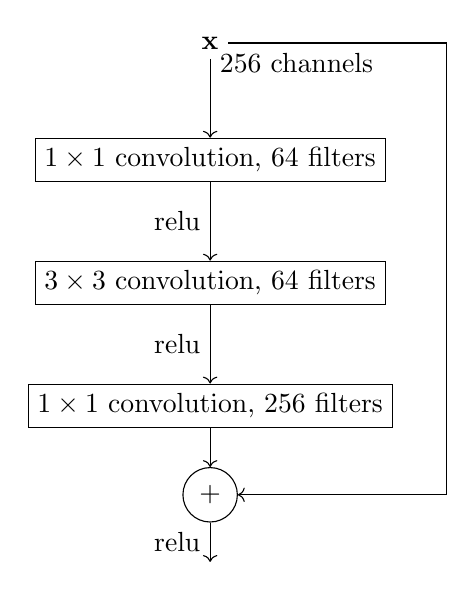
\begin{tikzpicture}
      \node[rectangle, draw] at (0, 0) (layer0)
        {$1\times1$ convolution, 64 filters};
      \node[rectangle, draw, below=1 of layer0] (layer1)
        {$3\times3$ convolution, 64 filters};
      \node[rectangle, draw, below=1 of layer1] (layer2)
        {$1\times1$ convolution, 256 filters};
      \node[circle, draw, below=.5 of layer2] (layer_add) {$+$};
      \node[below=.5 of layer_add] (layer_out) {};
      \node[above=1 of layer0] (layer_in)
        {$\mathbf{x}$};

      \draw[->] (layer_in) -- (layer0);
      \draw[->] (layer0) -- node[left]{relu} (layer1);
      \draw[->] (layer1) -- node[left]{relu} (layer2);
      \draw[->] (layer2) -- (layer_add);
      \draw[->] (layer_add) -- node[left]{relu} (layer_out);

      \draw[->] (layer_in) node[below right] {256 channels} -| ($(layer_add) + (3,0)$) |- (layer_add);
    \end{tikzpicture}
  \end{center}
  \caption{Example of a residual block in ResNet-50.}
  \label{fig:resnet50_block}
\end{figure}

\begin{figure}
  \begin{center}
    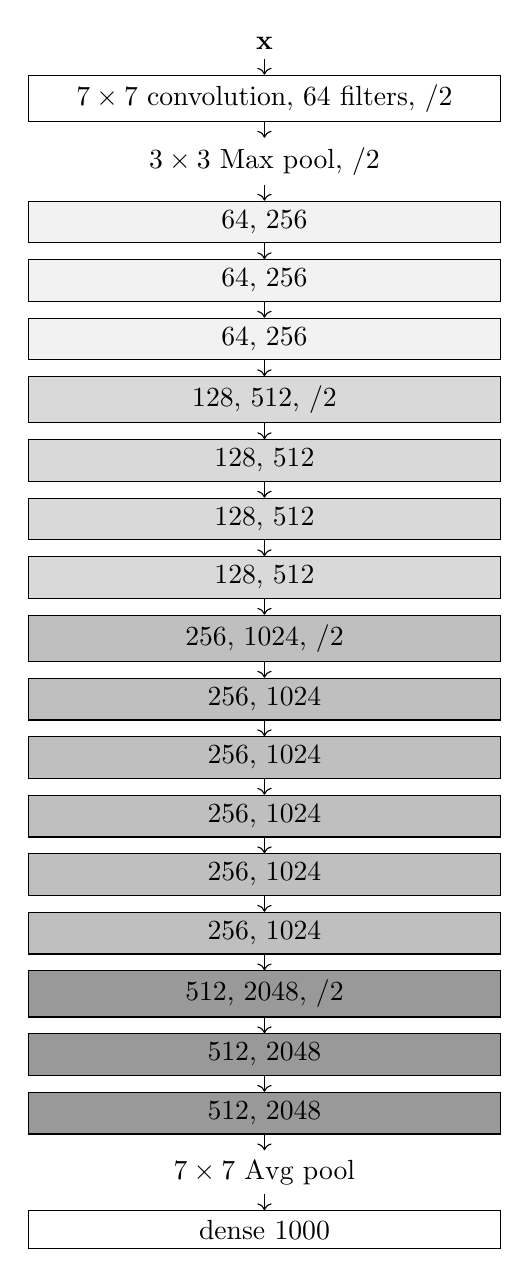
\begin{tikzpicture}[block/.style={rectangle, draw, minimum width=6cm}]
      \node[block, fill=black!5] at (0, 0) (block0) {64, 256};
      \node[block, fill=black!5, below=.2 of block0] (block1) {64, 256};
      \node[block, fill=black!5, below=.2 of block1] (block2) {64, 256};

      \node[block, fill=black!15, below=.2 of block2] (block3) {128, 512, /2};
      \node[block, fill=black!15, below=.2 of block3] (block4) {128, 512};
      \node[block, fill=black!15, below=.2 of block4] (block5) {128, 512};
      \node[block, fill=black!15, below=.2 of block5] (block6) {128, 512};

      \node[block, fill=black!25, below=.2 of block6] (block7) {256, 1024, /2};
      \node[block, fill=black!25, below=.2 of block7] (block8) {256, 1024};
      \node[block, fill=black!25, below=.2 of block8] (block9) {256, 1024};
      \node[block, fill=black!25, below=.2 of block9] (block10) {256, 1024};
      \node[block, fill=black!25, below=.2 of block10] (block11) {256, 1024};
      \node[block, fill=black!25, below=.2 of block11] (block12) {256, 1024};

      \node[block, fill=black!40, below=.2 of block12] (block13) {512, 2048, /2};
      \node[block, fill=black!40, below=.2 of block13] (block14) {512, 2048};
      \node[block, fill=black!40, below=.2 of block14] (block15) {512, 2048};

      \node[below=.2 of block15] (pool2) {$7\times7$ Avg pool};
      \node[block, below=.2 of pool2] (dense) {dense 1000};

      \node[above=.2 of block0] (pool1) {$3 \times 3$ Max pool, /2};
      \node[block, above=.2 of pool1] (conv1)
        {$7\times7$ convolution, 64 filters, /2};
      \node[above=.2 of conv1] (x) {$\mathbf{x}$};

      \draw[->] (block0) -- (block1);
      \draw[->] (block1) -- (block2);
      \draw[->] (block2) -- (block3);
      \draw[->] (block3) -- (block4);
      \draw[->] (block4) -- (block5);
      \draw[->] (block5) -- (block6);
      \draw[->] (block6) -- (block7);
      \draw[->] (block7) -- (block8);
      \draw[->] (block8) -- (block9);
      \draw[->] (block9) -- (block10);
      \draw[->] (block10) -- (block11);
      \draw[->] (block11) -- (block12);
      \draw[->] (block12) -- (block13);
      \draw[->] (block13) -- (block14);
      \draw[->] (block14) -- (block15);

      \draw[->] (x) -- (conv1);
      \draw[->] (conv1) -- (pool1);
      \draw[->] (pool1) -- (block0);
      \draw[->] (block15) -- (pool2);
      \draw[->] (pool2) -- (dense);
    \end{tikzpicture}
  \end{center}
  \caption{Schema of ResNet-50. Each block in the middle represents
    one residual block shown in Figure~\ref{fig:resnet50_block}.
    The first number shows the amount of filters the first two layers
    of a block have, while the second number shows the filters of the
    last layer of the block. $/2$ indicates that a stride of two is
    applied (spatial dimensions are halved---each convolutional and
    pooling layer has ``same'' padding). Whenever the filters are
    doubled (indicated by the varying grey scales), the shortcut layer
    is linearly projected to match the higher channels.}
  \label{fig:resnet50}
\end{figure}

% }}}


\subsection{SpiNNaker as a Neuromorphic Computer Architecture} % {{{
\label{subsec:intro_spinn}

Spiking Neural Network Architecture (SpiNNaker, for short) is a
massively parallel neuromorphic computer system designed to run
spiking neural networks with up to one billion neurons (and a trillion
synapses) in real-time \citep{painkras_et_al_2013}.
As stated in Section~\ref{sec:intro}, neuromorphic computing is
the approach of developing hardware inspired by the biological
nervous system \citep{mead_1989}.
Today, neuromorphic computer architectures range from very fast and
energy efficient but inflexible direct electronic models
(neurons in hardware) \citep{indiveri_et_al_2011} to very flexible but
energy demanding systems based on common consumer hardware and
software (neurons in software) \citep{plesser_et_al_2007}.
SpiNNaker sits somewhere in between.
On the one hand, flexibility is achieved by implementing neurons in
software.
On the other hand, speed is achieved by massive-parallelism and
energy efficiency by using energy efficient processors, rather than
fast ones \citep{furber_et_al_2020}.

The SpiNNaker system's basic building block is the SpiNNaker chip,
a multiprocessor chip consisting of 18 ARM968 cores and a
Network-on-Chip (NoC) system for communication between the cores
\citep{furber_et_al_2007, furber_et_al_2020}.
Each core can run up to 1000 spiking neurons, which communicate with
each other over spikes---small packages with a maximum size of 72 bits
which are sent over the NoC \citep{furber_et_al_2007, spinnaker_2020}.
Each core has a 64 Kb DTCM---data tightly-coupled memory---for the
application data and fast access to it.
The 32 Kb ITCM stores the instructions executed by the core
\citep{furber_et_al_2020}.
All cores on a chip share access to 128 Mb SDRAM---synchronous
dynamic random access memory---which has a higher capacity than
DTCM but is also a lot slower
\citep{furber_et_al_2020, spinnaker_2020a}.

By today's standards 18 cores do not qualify as a massively-parallel
system.
Therefore, a SpiNNaker machine consists of multiple chips connected
together in a 2D triangular (six edges per router instead of four)
torus \citep{furber_et_al_2020}.
The biggest SpiNNaker machine is the SpiNNaker1M supercomputer in
Manchester with over one million cores.
The SpiNNaker1M consists of 10 cabinets, each with five card frames
holding 24 SpiNN-5 boards.
A SpiNN-5 board has 48 SpiNNaker chips, which means the SpiNNaker1M
has 1,036,800 theoretical cores, assuming no faulty cores
\citep{furber_et_al_2020}.

SpiNNaker is quite different from common deep learning accelerators,
like general purpose graphics processing units (GPGPUs) or Google's
TPU \citep{jouppi_et_al_2017}.
Common deep learning libraries like Tensorflow
\citep{abadi_et_al_2015}, Keras \citep{keras} or PyTorch
\citep{paszke_et_al_2019} implement
deep learning on a layer basis, which means by multiplying
\textit{tensors} ($n$D arrays), rather than implementing deep learning
on a neuron level \citep{goodfellow_et_al_2016}.
Therefore, the common industry approach to building hardware
accelerators for deep learning is to facilitate fast matrix
multiplication, which represents the majority of computation needed
for training and inference.
The leading systems, when it comes to throughput and speed according
to the MLPerf training benchmark \citep{mlperf_2019}, are Google's
TPU \citep{jouppi_et_al_2017} and NVIDIA's GPU architecture
Volta \citep{durant_et_al_2017}.
Volta's successor Ampere was released in 2020, which, according to
NVIDIA, is much more powerful \citep{krashinsky_et_al_2020}.
Both architectures leverage instruction level parallelism, sacrificing
significant chip space for specialized units performing a
fused multiply-add-accumulate matrix operation (MAC).
NVIDIA calls these units tensor cores. The Tesla V100 has 640 tensor
cores, each performing one $4\times 4$ MAC per clock cycle, a
theoretical peek performance of 125 terraflop/s
\citep{markidis_et_al_2018}.
The TPUv1 comes with $256\times256$ MACs performing 8 bit (unsigned)
integer operations \citep{jouppi_et_al_2017}.
The TPUv2 added support for mixed precision floating point operations
(16 bit multiply with 32 bit add and accumulate, same as the
tensor core of the Volta architecture)
\citep{kennedy_2017, markidis_et_al_2018}.
The SpiNNaker cores do not have a MAC unit, being designed to run
spiking neurons efficiently, rather than lots of matrix
multiplications.
That means the prototype presented in Section~\ref{sec:SpiDNN} must
put more focus on leveraging SpiNNaker's massive parallelism, rather
than relying on fast instruction level parallelism.
For example with optimized domain decomposition and smarter algorithms
than matrix multiplication.

% }}}

% }}}


\section{Related Work} % {{{
\label{sec:related_work}

Like \citet{gomes_2017} states, implementing deep learning on
neuromorphic chips has been a desire for some time.
This section will outline two approaches of implementing deep learning
models on neuromorphic hardware.
One being the SNN toolbox \citep{rueckauer_et_al_2017}, the other
being an implementation of CNNs on IBM's TrueNorth system
\citep{esser_et_al_2016}.

The SNN toolbox takes pre-trained deep learning models and translates
them into spiking neural networks.
Its front-end supports a wide range of different input formats from
various deep learning libraries, including Keras, Tensorflow, PyTorch
or Caffe \citep{jia_et_al_2014}, while its back-end supports different
spiking neural network simulators like Brian2
\citep{stimberg_et_al_2019}, the simulator independent language PyNN
\citep{davison_et_al_2009} or direct mappings to neuromorphic
computers like SpiNNaker or Intel's Loihi
\citep{davies_et_al_2018, snn_toolbox_2020}.
It supports complex CNNs like VGG16 or Inception-v3
\citep{szegedy_et_al_2015, rueckauer_et_al_2017}.
\citet{rueckauer_et_al_2017} shows that using the converted version of
LeNet \citep{lecun_et_al_1989} on the MNIST data set
\citep{lecun_et_al_2020} and BinaryNet \citep{courbariaux_et_al_2016}
on CIFAR-10 \citep{krizhevsky_2009} requires two times
less operations than the original CNNs without considerable loss in
accuracy.
Unfortunately for bigger problems, namely VGG16 and Inception-v3 on
the ImageNet data set, the converted models have a much lower accuracy
than their original counterpart (63.9 percent accuracy for the
original VGG16 and only an accuracy of 49.6 for the converted model)
\citep{rueckauer_et_al_2017}.
Another caveat of the SNN toolbox is the fact that it only supports
inference and not training, which is the far more complex task
computationally.

IBM's TrueNorth neuromorphic architecture has the goal of
achieving energy efficiency and performance through scalability,
same as SpiNNaker.
\citet{esser_et_al_2016} presents Eedn (energy-efficient deep
neuromorphic networks).
Eedn is an approach of generating CNNs on the TrueNorth system,
enabling both inference and training.
TrueNorth---unlike SpiNNaker---uses one bit spikes
\citep{esser_et_al_2016}, which means its substantially different from
contemporary consumer hardware and deep learning accelerators and Eedn
is needed to translate the CNN in order to make it run on TrueNorth.
SpiNNaker on the other hand, like stated above, is just a collection
of low power ARM cores connected over a NoC.
Spikes on SpiNNaker a communicated with small multicast packets
(up to 72 bits, see above) \citep{furber_et_al_2020}.
These packets can be used to transfer any information from one core
to another.
This makes it much easier to implement deep learning on SpiNNaker,
because focus lies more on how to deconstruct the model and map it
onto the cores, rather than having to translate the model into a
SpiNNaker-specific format.
Nonetheless, Eedn models show promising results.
\citet{esser_et_al_2016} presents tests on 6 well known,
industry-strength data sets with the Eedn models having approximately
the same accuracy as the original models.
The throughput of the TrueNorth system is promising as well.
\citet{esser_et_al_2016} shows that TrueNorth is able to process
between 1,200 and 2,600 $32\times32\times3$ images per second.

% }}}


\section{Deep Learning on SpiNNaker} % {{{
\label{sec:SpiDNN}

This section will describe the developed deep learning prototype in
detail.
While Section~\ref{subsec:intro_spinn} gave a short overview over the
SpiNNaker hardware, Section~\ref{subsec:spinn_toolchain} will present
a short introduction to the SpiNNaker software toolchain and
programming model.
Section~\ref{subsec:SpiDNN_arch} will present the architecture of the
prototype.
Lastly, Section~\ref{subsec:problems} will shine light onto the
hardships and problems encountered and mistakes made during the
development process.


\subsection{The SpiNNaker Programming Model} % {{{
\label{subsec:spinn_toolchain}

Parallel programming is hard \citep{lee_2011}, especially on novel
hardware architectures like SpiNNaker \citep{brown_et_al_2015}.
SpiNNaker provides layers of software abstractions over the hardware
to make programming and exploiting the capabilities of it as easy as
possible \citep{furber_et_al_2020}.

The SpiNNaker hardware is designed to tackle problems which can be
decomposed into many small, autonomous units without a central
computational overseer \citep{brown_et_al_2015}.
These problems are commonly known as embarrassingly parallel problems
\citep{foster_1995}.
The software toolchain lets the user describe their program as a
graph.
Each vertex of the graph represents one unit of computation
(e.g.\ a bunch of spiking neurons or a perceptron in our case)
and directed edges represent the communication between the units
\citep{furber_et_al_2020}.

There are two type of graphs, application graphs and machine graphs.
A vertex in the machine graph---a machine vertex---is directly mapped
to a single SpiNNaker core.
An application graph is an abstraction over a machine graph.
Application vertices have atoms.
Atoms are atomic units of computation.
The atoms of an application vertex are distributed onto machine
vertices.
This makes programming and scaling easier and also facilitates proper
resource exploitation, for example by mapping 1,000 small spiking
neurons---atoms of a neuron population represented as a application
vertex---onto a single core, instead of having them distributed across
1,000 cores, which would be the case if they were to be implemented
directly as machine vertices \citep{furber_et_al_2020}.
For the prototype we used a machine graph, since it is easier to
implement.
The development process was guided by the UNIX rule of optimization:
prototype before polishing \citep{raymond_2003}, or in Donald Knuth's
words: ``premature optimization is the root of all evil''
\citep{knuth_1974}.

The toolchain is written in the Python programming language.
The SpiNNaker machine is connected to a host device via Ethernet
\citep{rowley_et_al_2019}.
The toolchain---running on the host---is mainly responsible for
the generation of the graph and its execution on the connected
SpiNNaker machine.
It goes through a stage of mapping the graph onto the available cores,
before data generation (where e.g.\ parameters of the vertex are
loaded into SDRAM) and finally running the application
\citep{furber_et_al_2020}.

Each vertex is represented as a Python object---instantiated from the
appropriate classes---and has an associated binary, the program to
be executed by the machine \citep{furber_et_al_2020}.
The source code of the binary to be executed on the machine is written
in the C programming language and compiled with the gcc compiler from
the GNU ARM embedded toolchain \citep{arm_2020, rowley_et_al_2019}.
Machine vertices are not common C programs.
They do not own the control flow but instead are event-based, like
the ECMAScript programming language \citep{ecma_2020}.
The SpiNNaker1 API provides the operating system executing the vertex
and serves the mechanism for registering software callback functions,
triggered when a certain event occurs \citep{furber_et_al_2020}.
The two events used by the vertices of this prototype were:
(\romannumeral 1) receiving a packet and (\romannumeral 2) a
periodical update event, called every $x$ cycles.

\begin{figure} % {{{
\begin{center}
  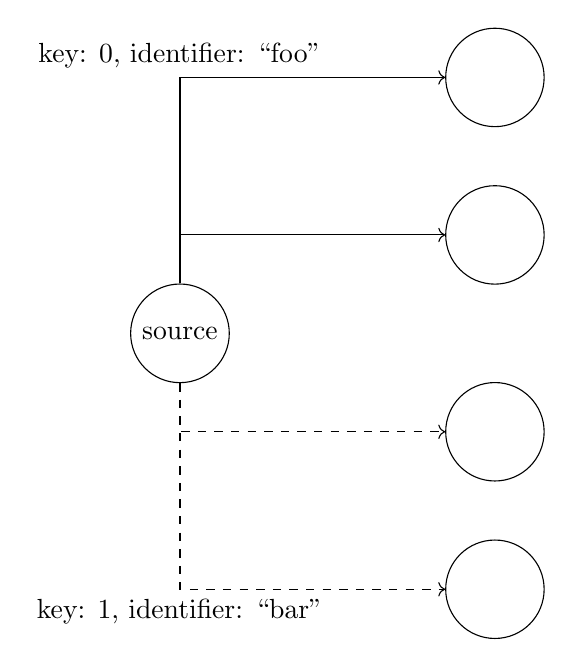
\begin{tikzpicture}[dot/.style={circle, draw, minimum size=1.25cm}]
    \node[dot] at (0, 0) (source) {source};

    \node[dot] at (4, 3.25) (dest1) {};
    \node[dot] at (4, 1.25) (dest2) {};
    \node[dot] at (4, -1.25) (dest3) {};
    \node[dot] at (4, -3.25) (dest4) {};

    \draw[->] (source) |-
      node[above]{key: 0, identifier: ``foo''} (dest1);
    \draw[->] (source) |- (dest2);

    \draw[->, dashed] (source) |- (dest3);
    \draw[->, dashed] (source) |-
      node[below]{key: 1, identifier: ``bar''} (dest4);
  \end{tikzpicture}
\end{center}
\caption{Example of a machine vertex ``source'' connected to four
  other machine vertices over two outgoing edge partitions. If the
  source vertex sends a MC packet with zero as key, the two upper
  vertices will receive the packet, whereas with one as key the two
  lower vertices would receive the packet.}
\label{fig:partitions}
\end{figure} % }}}

Machine vertices communicate with each other via MC (multicast)
packets.
A MC packet has two or three segments:
(\romannumeral 1) one control byte, (\romannumeral 2) 4 byte key
and (\romannumeral 3) optionally 4 byte payload.
This makes a MC packet either 40 or 72 bits long
\citep{furber_et_al_2020}.
A MC packet is send via the directed edges between vertices.
Each edge has an associated outgoing edge partition.
An outgoing edge partition has one source vertex and $n$ destination
vertices and---in the case of the machine graph---one unique
routing key (allocated by the toolchain).
The routing key---a 32 bit unsigned integer---is unique in the sense
that no other outgoing edge partition will have the same key.
Otherwise routing would fail in the sense that packets will be send
to the wrong destinations.
If the source vertex sends a MC packet it uses the key of the
outgoing edge partition.
The packet will reach all destination vertices of the partition.
A vertex can have multiple outgoing edge partitions
(see Figure~\ref{fig:partitions}) \citep{furber_et_al_2020}.

The toolchain offers support for live IO, enabling external devices
(like robots, or in our case the host) to interact with the
application running on SpiNNaker.
Interaction happens, again, via MC packets and by adding extra
vertices for input and output to the graph.
Live input is enabled by the \texttt{ReverseIPTagMulticastSource}
(RIPTMCS) machine vertex and live output by the
\texttt{LivePacketGatherer} (LPG) \citep{furber_et_al_2020}.
The toolchain provides a \texttt{LiveEventCon\-nection} for the
external device, which supplies the appropriate abstractions over the
networking.
Like the SpiNNaker1 API, the \texttt{Live\-Event\-Con\-nection}
provides an event-based interface with callbacks.

% }}}


\subsection{The Prototype} % {{{
\label{subsec:SpiDNN_arch}

The underlying assumption made for developing the prototype was,
that because SpiNNaker was designed to run spiking neurons, it would
be a natural fit to implement deep learning on a neuron level as well.
Besides that, neurons are an easy-to-understand abstraction over the
mechanisms of deep learning and rather straight-forward to implement.
This design decision was made against the trend of both deep learning
research and state-of-the-art deep learning libraries.
The former more commonly abstracts over layers while the latter
implements deep learning as a computational graph
\citep{goodfellow_et_al_2016}.
Problems with this assumption are discussed in
Section~\ref{subsec:problems}.
The API of the prototype was designed to resemble the API of the Keras
deep learning library \citep{keras}.
An example comparison can be seen in
Listing~\ref{lst:spiDNN_vs_keras}.


\begin{figure} % {{{
\begin{lstlisting}[language=Python, caption={Example code comparing
  Keras to the prototype. The code would result in a model akin to the
  one shown in Figure~\ref{fig:spiDNN_arch}.}, captionpos=b,
  label=lst:spiDNN_vs_keras, numbers=left]
import tensorflow as tf
import numpy as np

# prototype library
from spiDNN import Model
from spiDNN.layers import Input, Dense

# random test set
X = np.random.rand(500, 64)

# the keras model
keras_model = tf.keras.Sequential()
keras_model.add(tf.keras.layers.Dense(128, input_shape=(64,)))
keras_model.add(tf.keras.layers.Dense(128, activation="relu"))
keras_model.add(tf.keras.layer.Dense(10, activation="softmax"))

# the equivalent model for SpiNNaker
spinn_model = Model()
spinn_model.add(Input(64))
spinn_model.add(Dense(128))
spinn_model.add(Dense(128, activation="relu"))
spinn_model.add(Dense(10, activation="softmax"))

# this call ensures both models have the same parameters
model.set_weights(keras_model.get_weights())

# predict the results for the random test set
# (with random weights)
p_ = kmodel.predict(X)
p = model.predict(X)

error = np.absolute(p - p_)

# difference in prediction can happen,
# due to floating point errors
assert np.amax(error) < 1e-4
\end{lstlisting}
\end{figure} % }}}

The prototype exposes the \texttt{Model} class to the user.
The model is the main interface to SpiNNaker and---as the name
clearly suggests---functions as the representation of a deep learning
model.
It is designed to be used the same way as Keras's \texttt{Sequential}
model (see Listing~\ref{lst:spiDNN_vs_keras}).
The second user interface are the layers---the building blocks of
a model.
Layers are added sequentially to a model instance by calling the
model's \texttt{add} method.
A layer has at most one preceding and one succeeding layer
(see Figure~\ref{fig:spiDNN_arch}).
While this suits most common needs, modern deep learning models,
like the inception nets \citep{szegedy_et_al_2014}, have layers
connected to multiple preceding and succeeding layers.
Also the shortcut connections of the ResNets (see
Section~\ref{subsec:intro_bench}) are not straight forward to
implement with the sequential API.
Keras therefore exposes another API, its functional API.
The prototype was not developed so far and only supports sequential
models.

The model stores the trainable parameters (the weights of the layers),
which can be accessed via the \texttt{set\_weights} and
\texttt{get\_weights} methods of the model class.
The parameters are generated during the \texttt{add} call by the
added layer, since weights are different for different layer types
and can depend on the preceding layer.
For example, a dense layer generates the weight matrix
$\mathbf{W}: n \times m$ and the bias $m$-vector.
$n$ is the amount of neurons in the preceding layer, $m$ the amount of
neurons of the dense layer.
Convolutional layers do not depend on the previous layer for their
weights.
For example a 1D convolutional layer generates a $3$D array
$\mathbf{W}: \text{\textit{kernel size}} \times channels \times
filters$ and a bias $filters$-vector.
$\mathbf{W}$ are the kernels for each filter (see
Section~\ref{subsec:intro_dl}).
The kernel of a 2D convolutional layer simply has one more spatial
dimension, so the 2D layer would generate a 4D array as weights.
The input layer does not generate any weights.
The formats of the weights is again inspired by Keras and enables
seamless interoperability between a SpiNNaker deep learning model and
the subset of the Keras API supported by the prototype
(see Listing~\ref{lst:spiDNN_vs_keras}, line 25).
Having our prototype so closely resemble Keras had the great advantage
of enabling precise integration testing.
We could simply build two equal models, one in Keras and one with our
prototype, and compare their outputs against each other
(see Listing~\ref{lst:spiDNN_vs_keras}, lines 29ff).
The same goes for testing backpropagation, where we could simply train
both models and compare the updated weights.

\begin{figure} % {{{
  \begin{center}
    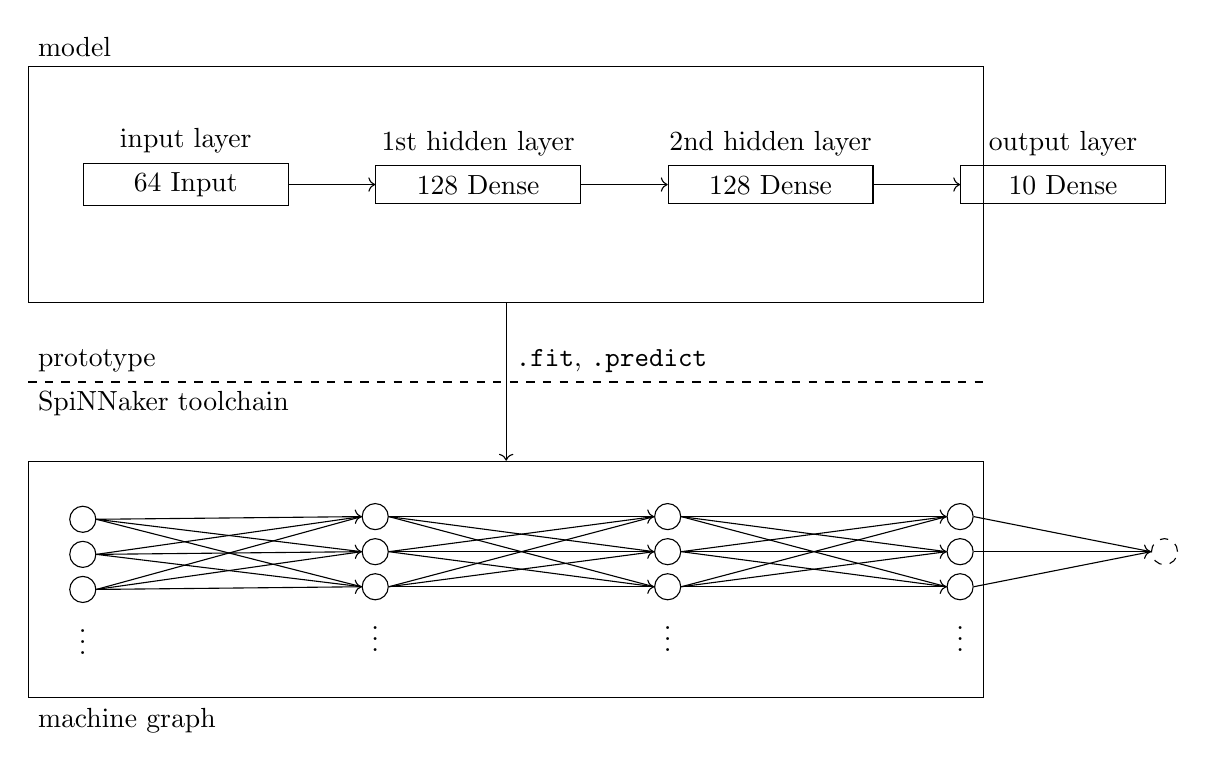
\begin{tikzpicture}[
      elem/.style={rectangle, draw},
      dot/.style={circle, draw},
      layer/.style={minimum width=2.6cm},
      container/.style={minimum width=\linewidth,
                         minimum height=3cm}
    ]
      \node[elem, container]
        at (0, 0) (model) {};
      \node[above right] at (model.north west) {model};

      \node[elem, layer, label=input layer]
        (layer_input) at ($(model.west) + (2, 0)$) {64 Input};
      \node[elem, layer, label=1st hidden layer, right=1.1 of layer_input]
        (layer_hidden1) {128 Dense};
      \node[elem, layer, label=2nd hidden layer, right=1.1 of layer_hidden1]
        (layer_hidden2) {128 Dense};
      \node[elem, layer, label=output layer, right=1.1 of layer_hidden2]
        (layer_output) {10 Dense};

      \draw[->] (layer_input) -- (layer_hidden1);
      \draw[->] (layer_hidden1) -- (layer_hidden2);
      \draw[->] (layer_hidden2) -- (layer_output);


      \draw[dashed] ($(model.south west) - (0, 1)$)
        node[above right] {prototype}
        node[below right] {SpiNNaker toolchain} --
        ($(model.south east) - (0, 1)$);

      \node[elem, container, below=2 of model] (machine_graph) {};
      \node[below right] at (machine_graph.south west)
        {machine graph};

      \node[dot, below=3.8 of layer_input.south west]
        (input0) {};
      \node[dot, below=.1 of input0]
        (input1) {};
      \node[dot, below=.1 of input1]
        (input2) {};
      \node[below=.001 of input2] {\vdots};

      \node[dot, below=3.8 of layer_hidden1.south west]
        (hidden00) {};
      \node[dot, below=.1 of hidden00]
        (hidden01) {};
      \node[dot, below=.1 of hidden01]
        (hidden02) {};
      \node[below=.001 of hidden02] {\vdots};

      \node[dot, below=3.8 of layer_hidden2.south west]
        (hidden10) {};
      \node[dot, below=.1 of hidden10]
        (hidden11) {};
      \node[dot, below=.1 of hidden11]
        (hidden12) {};
      \node[below=.001 of hidden12] {\vdots};

      \node[dot, below=3.8 of layer_output.south west]
        (output0) {};
      \node[dot, below=.1 of output0]
        (output1) {};
      \node[dot, below=.1 of output1]
        (output2) {};
      \node[below=.001 of output2] {\vdots};


      \node[dot, dashed, right=2.25 of output1] (lpg) {};


      \draw[->] (model) -- node[above right]
        {\texttt{.fit}, \texttt{.predict}} (machine_graph);

      \draw[->] (input0.east) -- (hidden00.west);
      \draw (input0.east) -- (hidden01.west);
      \draw (input0.east) -- (hidden02.west);

      \draw (input1.east) -- (hidden00.west);
      \draw[->] (input1.east) -- (hidden01.west);
      \draw (input1.east) -- (hidden02.west);

      \draw (input2.east) -- (hidden00.west);
      \draw (input2.east) -- (hidden01.west);
      \draw[->] (input2.east) -- (hidden02.west);

      \draw[->] (hidden00.east) -- (hidden10.west);
      \draw (hidden00.east) -- (hidden11.west);
      \draw (hidden00.east) -- (hidden12.west);

      \draw (hidden01.east) -- (hidden10.west);
      \draw[->] (hidden01.east) -- (hidden11.west);
      \draw (hidden01.east) -- (hidden12.west);

      \draw (hidden02.east) -- (hidden10.west);
      \draw (hidden02.east) -- (hidden11.west);
      \draw[->] (hidden02.east) -- (hidden12.west);

      \draw[->] (hidden10.east) -- (output0.west);
      \draw (hidden10.east) -- (output1.west);
      \draw (hidden10.east) -- (output2.west);

      \draw (hidden11.east) -- (output0.west);
      \draw[->] (hidden11.east) -- (output1.west);
      \draw (hidden11.east) -- (output2.west);

      \draw (hidden12.east) -- (output0.west);
      \draw (hidden12.east) -- (output1.west);
      \draw[->] (hidden12.east) -- (output2.west);

      \draw (output0.east) -- (lpg.west);
      \draw[->] (output1.east) -- (lpg.west);
      \draw (output2.east) -- (lpg.west);
    \end{tikzpicture}
  \end{center}
  \caption{Illustration of how a machine graph is generated by the
    prototype. The dashed circle represents an auxiliary machine
    vertex, in this case the LPG. This machine graph would be
    generated when the \texttt{predict} method of the model is
    called.}
  \label{fig:spiDNN_arch}
\end{figure} % }}}

Supported layers are: (\romannumeral 1) input,
(\romannumeral 2) dense and (\romannumeral 3) 1D convolutional layers.
A flatten layer (used for flattening a feature map into a one
dimensional vector so it can be processed by a dense layer) is
implicitly implemented (see Listing~\ref{lst:spiDNN_vs_keras_cnns}).
Besides layers, the prototype supports the following activation
functions:
\begin{itemize}
  \item identity (default when activation unspecified): $f(x) = x$.
  \item tanh: $f(x) = tanh(x)$
  \item sigmoid: $f(x) = \frac{1}{1 + \exp(-x)}$
  \item relu (rectified linear unit): $f(x) = max(0, x)$
  \item softmax: $f(x_i) = \frac{\exp(x_i)}{\sum_{j=1}^{N}\exp(x_j)}$
\end{itemize}
The only supported optimizer (algorithm for training the weights) is
gradient descent with a constant learning rate.
Gradient descend is probably the most common optimization algorithm
for deep learning \citep{goodfellow_et_al_2016}.
1D convolutional layers have support for same and valid (default)
padding and they can be strided (see Section~\ref{subsec:intro_dl}).

\begin{figure} % {{{
\begin{lstlisting}[language=Python, caption={Example code comparing
  1D CNNs in Keras to the prototype.}, captionpos=b,
  label=lst:spiDNN_vs_keras_cnns, numbers=left]
import tensorflow as tf
import numpy as np

# prototype library
from spiDNN import Model
from spiDNN.layers import Input, Dense, Conv1D

# 64 features, each with 4 channels
input_shape = (64, 4)

# random test set
X = np.random.rand(500, *input_shape)

# the keras model
keras_model = tf.keras.Sequential()
# this layer has 20 filters and a kernel size of 3
keras_model.add(tf.keras.layers.Conv1D(20, 3, input_shape=input_shape))
keras_model.add(tf.keras.layers.Conv1D(5, 3, activation="relu"))
keras_model.add(tf.keras.layers.Flatten())
keras_model.add(tf.keras.layer.Dense(10, activation="softmax"))

# the equivalent model for SpiNNaker
spinn_model = Model()
spinn_model.add(Input(*input_shape))
spinn_model.add(Conv1D(20, (3,)))
# The feature map of this layer is implicitly flattened,
# because the next layer is a dense layer
spinn_model.add(Conv1D(5, (3,), activation="relu"))
spinn_model.add(Dense(10, activation="softmax"))

# this call ensures both models have the same parameters
model.set_weights(keras_model.get_weights())

# predict the results for the random test set
# (with random weights)
p_ = kmodel.predict(X)
p = model.predict(X)

error = np.absolute(p - p_)

# difference in prediction can happen,
# due to floating point errors
assert np.amax(error) < 1e-4
\end{lstlisting}
\end{figure} % }}}

Like stated above, a deep learning model is decomposed into neurons
in order to execute it on SpiNNaker.
Neurons are part of the internal APIs of the prototype and not exposed
to the user.
The neuron of a dense layer can be seen in
Figure~\ref{fig:perceptron}.
Each neuron of a convolutional layer performs one single convolution
operation with all filters of the layer.
For example, when we look at Figure~\ref{fig:conv_op}, $ax + by + cz$
would be one convolution with one filter.
If the layer has a second filter with a kernel $w, v, u$, the neuron
would produce a second value $aw + bv + cu$.
The input $a, b, c$ stays the same.
A convolutional layer is schematized in Figure~\ref{fig:cnn}.

Figure~\ref{fig:spiDNN_arch} shows how to operate the prototype.
The user defines the sequential deep learning model, like described
above.
Only when the inference or training operations are called is the
model translated into a SpiNNaker machine graph and executed on the
connected machine.
For inference one has to call the \texttt{predict} method of the
model and for training the \texttt{fit} method.

Algorithm~\ref{alg:pred} shows what happens during the
\texttt{predict} method.
First, an auxiliary layer for the live IO is created, the extractor
layer.
The extractor layer has a single machine vertex, a LPG instance
(see Section~\ref{subsec:spinn_toolchain}) for streaming the
predictions off of SpiNNaker, back to the host.
The first layer---which must always be an input layer---handles
streaming the data onto the machine.
Neurons of a input layer are simple wrappers around the RIPTMCS
machine vertices provided by the SpiNNaker toolchain (see
Section~\ref{subsec:spinn_toolchain}).

The layer interface specifies a \texttt{reset} method, which is
called for each layer in Algorithm~\ref{alg:pred}, line 2.
This method resets the neurons of a layer (simply deletes them).
If, for example, the model was trained before the call to the
\texttt{predict} method---probably the most common workflow in deep
learning---the neurons from the training graph would still exist.
Beyond the training these neurons are meaningless, because they were
part of a different run on SpiNNaker and must be deleted (when the
toolchain is resetted it deletes its machine graph instance, but the
vertex objects remain).
They could be deleted right before the \texttt{fit} or
\texttt{predict} method exits, but for unit testing it is convenient
to still have the neurons beyond a run on SpiNNaker.

After the machine and the SpiNNaker toolchain are set up, the
machine vertices (neurons) are initialized
(see Algorithm~\ref{alg:pred}, line 4).
The layer interface always sits between the model and the neurons.
The model only ever calls methods of the layers.
This is a design pattern in software engineering called the layered
pattern (not to be confused with the layers provided by our
prototype) \citep{morlion_2018}.
This design pattern is a common way to abstract---e.g.\ TCP/IP or the
OSI model \citep{tanenbaum_et_al_2013}---and holds code complexity
down, makes ownership clear and helps writing well-defined interfaces.
For the initialization of the neurons, the layer interface provides
a method \texttt{init\_neurons}.
This method generates the neurons, which are stored in the
\texttt{neurons} property of each layer (a Python list).
The \texttt{init\_neurons} method furthermore adds the neurons to
the machine graph of the SpiNNaker toolchain.

After the neurons are created and initialized, the connections for
the forward pass are generated (see Algorithm~\ref{alg:pred}, lines 5
and 6).
The layer interface offers the \texttt{connect\_incoming} and
\texttt{connect\_outgoing} functions for this.
Incoming and outgoing refer to the called layer, respectively.
For example, the forward pass is built with calling
\texttt{connect\_incoming} for each hidden layer, the output layer
and the auxiliary layer for extracting the predictions.
Each of these layers is connected with the preceding layer.
All layers except convolutional layers connect every of their neurons
with every neuron of the layer connected with.
Connecting convolutional layers is more complicated, because they
also need to take care of stride and padding.

Last thing to be set up, before execution can start, is the live IO
connection for streaming the observations onto the board and the
predictions off it (see Algorithm~\ref{alg:pred}, line 7).
The communication protocol chosen was the most naive possible
solution, staying true to our development principle (see above).
We called the protocol ping-pong protocol, because the communication
pattern resembles table tennis, the host being one player, the
SpiNNaker machine the other.
The host always sends data onto the board (ping) and receives some
sort of result (pong).
After receiving the pong, another ping is sent by the host or the
execution is stopped when no more data is there to send.
During inference the observations are streamed onto the board as the
ping events.
The deep learning model processes each observation and returns the
predictions of the output layer as the pong event.
Each prediction is collected by the live IO callback function for
receiving data and returned from the \texttt{predict} method
(see Algorithm~\ref{alg:pred}, line 11).

The ping-pong protocol is easy to implement and easy to reason about.
Its main disadvantage is performance.
One can easily see the problem.
Only a single layer is processing an observation at a time.
All other layers wait.
This is a huge waste of time, especially for very deep model
architectures.
A possible solution to this problem is discussed in
Section~\ref{sec:discussion}.

\begin{algorithm} % {{{
  \caption{: \texttt{predict} method}
  \label{alg:pred}

  \begin{algorithmic}[1]
    \STATE{create extractor layer}
    \STATE{reset layers}
    \STATE{setup SpiNNaker}
    \STATE{initialize machine vertices}
    \STATE{establish forward pass connections}
    \STATE{establish connection between output layer and extractor}
    \STATE{setup live IO}
    \STATE{execute model on SpiNNaker (run forever)}
    \COMMENT{the live IO connection stops the execution}
    \STATE{stop the SpiNNaker machine}
    \STATE{close live IO}
    \RETURN{predictions}
    \COMMENT{predictions collected by live IO}
  \end{algorithmic}
\end{algorithm} % }}}

Like stated above, weights are actually owned by the model, not
the layer objects.
The weights are directly injected into the neurons during their
generation and initialization.
Conceptually, a perceptron (neuron of a dense layer) owns the weights
associated with its incoming connections.
The filters of the convolutional layers are simply shared between
all neurons of the layer, so each neuron has a copy.

How are received packets matched to the correct weight?
All packets send by the different components of the prototype are
with payload, so 72 bit big.
Each packet consists of a control byte and two words, key and payload
(see Section~\ref{subsec:spinn_toolchain}).
Each neuron knows how many neurons in the previous layer it is
connected to and knows their keys within a certain partition.
The simple MLP shown in Figure~\ref{fig:spiDNN_arch} only has a
single partition the ``forward'' partition\footnote{Not actually one
  partition, but lots of outgoing edge partitions with the same
  identifier (see Section~\ref{subsec:spinn_toolchain}).}.
During data generation (see Section~\ref{subsec:spinn_toolchain})
the SpiNNaker toolchain can be queried and the machine graph traversed
in order to find out the corresponding routing keys.
The routing keys of the outgoing edge partitions of all the neurons
from the previous layer, connected to the neuron which is creating its
mapping between packets and weights, are collected.
The keys are guaranteed to be consecutive.
For example, the first neuron of the input layer of the MLP from
Figure~\ref{fig:spiDNN_arch} would have zero as its key.
The second neuron one.
The first neuron of the first hidden layer would have 64 as key and so
forth.
How we changed the key allocation process to make this guarantee will
be discussed below.

After having collected the keys of the neurons from the previous
layer, the \textit{minimum key} is determined and passed as argument
to the machine vertex running on SpiNNaker.
The weights of the neuron are also passed as an argument to the
machine vertex.
The weights are a simple array of floats.
Now if a packet is received, the weight corresponding to the
connection is simply determined by indexing the weight array with the
index being the key of the received packet minus the minimum key.
The same procedure works for the backward pass as well.
For convolutional neurons it is somewhat more difficult, because they
receive multiple channels from their preceding neurons.
The index is therefore determined with an additional array of channel
counters.
For each connection a channel counter is created.
A channel counter is incremented each time a value is received from
its corresponding connection.
The channel counter is then additionally used to determine the correct
index of the weight the payload of the packet must be multiplied with.

% pseudo code for update and receive methods of the perceptron machine
% vertex



% then paragraph softmax

% softmax -> difficulties with partitions -> own partition manager

\begin{itemize}
  \item communication structure (partitions and global partition manager)
  \item backward pass
  \item graph structure (especially focused on edge and host--SpiNN
    communication)
  \item (Conv1D)
\end{itemize}

% }}}


\subsection{Problems} % {{{
\label{subsec:problems}

\begin{itemize}
  \item time
  \item mention problem with LPG
  \item what is all missing (2D, Pooling and Shortcut connections)
  \item Too much time spend in receive callback
  \item interpreting neurons as domain decomposition over linear algebra
    compute graph
  \item backward pass: gradients computed two times so comm fabric is
    not overly used by unique partitions/lots of unused packages
  \item How I crushed $n$d-kernels into a single blog of weights
  \item backprop design change (shared weights $\rightarrow$ redundant
    packets (easier and nicer to implement)).
    Really stress this point and present all three things tried
    (e-mail).
  \item resource invariance (first prototype, deemed too difficult
    to put resources into it as well (just three months time))
  \item bottlenecks (one layer much higher
    computational effort but even less resources (10--1024--20)
  \item conv neurons of resnet way too big and are horrific scalers
    (small spatial input but big channels computationally much more
    effort but again, less resources)
\end{itemize}

% }}}

% }}}


\section{Benchmark}
\label{sec:benchmark}

\section{Discussion}
\label{sec:discussion}

\begin{itemize}
  \item present possible solutions for problems encountered
  \item space used inefficiently (cores and memory) $\rightarrow$ better
    domain decomposition
  \item with this streaming model I have no easy way to do batch
    normalization---implications for vanishing/exploding gradients
    during training
  \item Ping-pong protocol sucks performance wise
\end{itemize}

\section{Conclusion}
\label{sec:conclusion}

\section{Next Steps}
\label{sec:next_steps}

\begin{itemize}
  \item profiling
  \item cost model
  \item multiple copies of the same network on the same machine
    $\rightarrow$ use all resources available
  \item better domain decomposition (SpiNNaker application graph or
    custom solution (application graph not helpful for neurons which
    become too big))
  \item smart algorithms vs.\ integrating with state-of-the-art libraries
    (investing time in stuff like SLIDE and the one paper by the Austrian
    guys about sparse connections explicitly mentioning SpiNNaker and
    neuromorphic chips or rather work on a trans-/compiler
    that efficiently translates linear algebra operations (like TF,
    PyTorch,\dots) onto SpiNNaker)
  \item integrate into compiler projects like Apache-TVM, XLA, Glow,
   nGraph, etc.
  \item implementing ONNX spec to make it easy for developers to use
    SpiNNaker (develop in PyTorch $\rightarrow$ run on SpiNNaker)
\end{itemize}

\bibliography{library.bib}
\addcontentsline{toc}{section}{References}

\end{document}
